\documentclass[12pt]{article}
\usepackage{times} 			% use Times New Roman font

\usepackage[margin=1in]{geometry}   % sets 1 inch margins on all sides
\usepackage{hyperref}               % for URL formatting
\usepackage[pdftex]{graphicx}       % So includegraphics will work
\setlength{\parskip}{1em}           % skip 1em between paragraphs
\usepackage{indentfirst}            % indent the first line of each paragraph
\usepackage{datetime}
\usepackage[small, bf]{caption}
\usepackage{listings}               % for code listings
\usepackage{xcolor}                 % for styling code
\usepackage{multirow}
\usepackage{xurl} 
\usepackage{enumitem}
\usepackage[section]{placeins}
\usepackage{float}
\usepackage{hyperref}

%New colors defined below
\definecolor{backcolour}{RGB}{246, 246, 246}   % 0xF6, 0xF6, 0xF6
\definecolor{codegreen}{RGB}{16, 124, 2}       % 0x10, 0x7C, 0x02
\definecolor{codepurple}{RGB}{170, 0, 217}     % 0xAA, 0x00, 0xD9
\definecolor{codered}{RGB}{154, 0, 18}         % 0x9A, 0x00, 0x12

%Code listing style named "gcolabstyle" - matches Google Colab
\lstdefinestyle{gcolabstyle}{
  basicstyle=\ttfamily\small,
  backgroundcolor=\color{backcolour},   
  commentstyle=\itshape\color{codegreen},
  keywordstyle=\color{codepurple},
  stringstyle=\color{codered},
  numberstyle=\ttfamily\footnotesize\color{darkgray}, 
  breakatwhitespace=false,         
  breaklines=true,                 
  captionpos=b,                    
  keepspaces=true,                 
  numbers=left,                    
  numbersep=5pt,                  
  showspaces=false,                
  showstringspaces=false,
  showtabs=false,                  
  tabsize=2
}

\lstset{style=gcolabstyle}      %set gcolabstyle code listing

\makeatletter
\g@addto@macro{\UrlBreaks}{\UrlOrds}
\makeatother

% for fancy page headings
\usepackage{fancyhdr}
\setlength{\headheight}{13.6pt} % to remove fancyhdr warning
\pagestyle{fancy}
\fancyhf{}
\rhead{\small \thepage}
\lhead{\small HW2, Lewis}  
\chead{\small CS 432, Fall 2020} 

%-------------------------------------------------------------------------
\begin{document}

\begin{centering}
{\large\textbf{HW2 - Web Archiving}}

Brenden Lewis\\                     
Due: 10/11/2020 11:59PM\\                      
\end{centering}

%-------------------------------------------------------------------------
\section*{Q1}
When observing Twitter posts through the API, I decided to opt for posts that contained the string 'Youtube' in an attempt to keep my scope to YouTube video links. The Tweepy and Request libraries were utilized to extract the links from each Twitter post. I was not able to figure out how to check for duplicate URIs in an efficient manner, but I was able to extract about 1,200 total links related to YouTube in some capacity. Each twitter post streamed in was parsed to JSON format for observation.

\par I did not keep an exact count of the number of shortened links that redirected elsewhere, but observing all the links I was collecting both in testing and in my final collection were largely comprised of redirecting links. I created a recursive function called \emph{def unshorten\textunderscore url(short \textunderscore url)} to "unshorten" these links and return the final destination after however many redirects are needed.

\par Due to this method being called for every link to ensure it is the final location, the connection to the API was often breaking due to the large amount of processing happening during the stream. In order to alleviate this issue, I had to collect the links in batches to ensure a stable connection; after a good deal of testing, I had the most consistent success with a maximum of 70 links collected in a single run. With each run of the program, I added the collected links to a text file \emph{TwitterURLs.txt}.

\lstinputlisting[language=Python, caption=Python code for Q1, label=lst:import]{q1.py}

\section*{Q2}
I opted to create a Python script to run MemGator from the command line for each link I had collected and return their TimeMaps in JSON format. To make creating the graphs easier after processing, I created a \emph{uri \textunderscore dict} dictionary for each entry containing the URI, number of mementos for that URI, and the age of its first memento. I capped my amount of processing at 1000 URIs worth of data. The program had to run continuously for about 10 hours to collect the TimeMap for each link; each link took an average of about 30s - 1:10 mins to process. After all URIs are processed, the program immediately creates several graphs from the data provided by the TimeMaps. Listing 3 shows the terminal output of the program which prints each URI dictionary and the total number of links processed and the number of links that had at least 1 memento.

\lstinputlisting[language=Python, caption=Python code for Q2 and Q3, label=lst:import]{q2.py}

\begin{lstlisting}[language=Python, caption=Terminal output after program execution, label=lst:copy]
{'uri': 'https://www.youtube.com/watch?v=5Zk_Vz-wz4g&feature=youtu.be\n', 'mementos': 0, 'age': 0}
{'uri': 'https://www.youtube.com/watch?v=bFUCiVcGK9g&feature=youtu.be\n', 'mementos': 1, 'age': 7}
{'uri': 'https://www.youtube.com/watch?v=3ej_bkYiQnE&feature=youtu.be\n', 'mementos': 0, 'age': 0}
{'uri': 'https://www.youtube.com/watch?v=Vm7l3YxEF8g&feature=youtu.be\n', 'mementos': 1, 'age': 2}
{'uri': 'https://www.youtube.com/watch?v=0zdS8hNM-sc&feature=youtu.be\n', 'mementos': 0, 'age': 0}
{'uri': 'https://exe.io/LgNUIAt\n', 'mementos': 0, 'age': 0}
{'uri': 'https://www.youtube.com/watch?v=5hfYJsQAhl0', 'mementos': 1361, 'age': 3871}

Total Urls: 1000

Total Urls w/ Mementos: 496
\end{lstlisting}

\par Listing 4 below shows the JSON output format for each link; this example in particular is from the very first link in the url text file. The program counts each memento listed under \emph{list} (if available) and the datetime of the first memento to calculate the age. The output for each link is stored collectively in a seperate textfile labeled \emph{timeMaps.txt}. The final size of this file came out to about 33MB, with many of the URIs having several thousands of mementos. 

\begin{lstlisting}[language=Python, caption=TimeMap of first link, label=lst:copy]
{
  "mementos": {
    "first": {
      "datetime": "2020-10-03T13:47:32Z",
      "uri": "https://web.archive.org/web/20201003134732/https://www.youtube.com/watch?v=4yAO5hbnfQQ&gl=US&hl=en"
    },
    "last": {
      "datetime": "2020-10-03T13:47:32Z",
      "uri": "https://web.archive.org/web/20201003134732/https://www.youtube.com/watch?v=4yAO5hbnfQQ&gl=US&hl=en"
    },
    "list": [
      {
        "datetime": "2020-10-03T13:47:32Z",
        "uri": "https://web.archive.org/web/20201003134732/https://www.youtube.com/watch?v=4yAO5hbnfQQ&gl=US&hl=en"
      }
    ]
  },
  "original_uri": "https://www.youtube.com/watch?v=4yAO5hbnfQQ",
  "self": "http://localhost:1208/timemap/json/https://www.youtube.com/watch?v=4yAO5hbnfQQ",
  "timegate_uri": "http://localhost:1208/timegate/https://www.youtube.com/watch?v=4yAO5hbnfQQ",
  "timemap_uri": {
    "cdxj_format": "http://localhost:1208/timemap/cdxj/https://www.youtube.com/watch?v=4yAO5hbnfQQ",
    "json_format": "http://localhost:1208/timemap/json/https://www.youtube.com/watch?v=4yAO5hbnfQQ",
    "link_format": "http://localhost:1208/timemap/link/https://www.youtube.com/watch?v=4yAO5hbnfQQ"
  }
}
\end{lstlisting}


\par Figures 1 and 2 below show histograms of the number of mementos from each URI and their frequency. Figure 1 shows the data from all URIs while Figure 2 attempts to show the same data excluding any URIs with 0 mementos. As also indicated in the program output, almost exactly half of the 1000 URIs observed had 0 mementos. Of the 496 links remaining, the large majority had very few mementos ranging between 1-100 mementos. Outside of a few outliers with thousands of mementos, most of the observed links are not well archived.   

\begin{figure}[H]
            \centering
            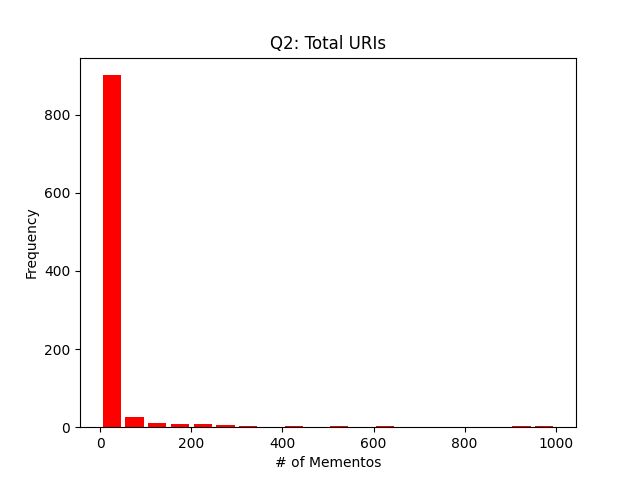
\includegraphics[width=0.95\textwidth]{Final_Histo_All_Data.png}
            \caption{Histogram showing the number of URIs vs. the number of mementos}
            \label{fig:my_label}
        \end{figure}

\begin{figure}[H]
            \centering
            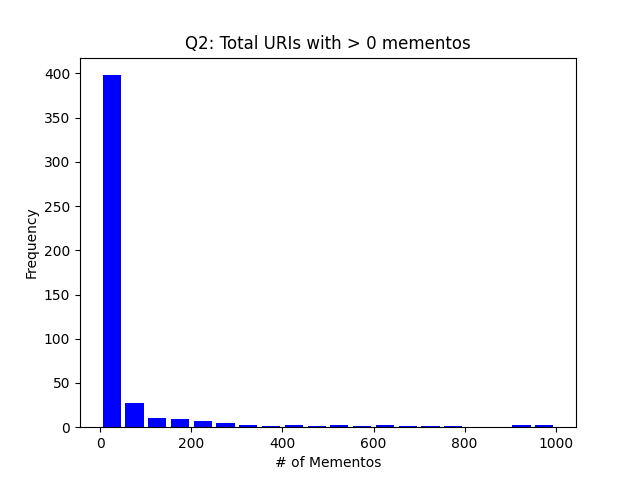
\includegraphics[width=0.95\textwidth]{Final_Histo_Above_Zero.png}
            \caption{Histogram showing the data from Figure 1 excluding URIs with no mementos}
            \label{fig:my_label}
        \end{figure}
        

\section*{Q3}

For each URI with non-zero memento counts, the age (in days) of the first memento is calculated through the \emph{def calculate \textunderscore age(output)} function that utilizes the \emph{datetime} library and takes the TimeMap of a URI in JSON as an argument. Figure 3 below is a scatterplot of all the URIs with non-zero mementos. Each URI is plotted by the number of mementos its TimeMap contains and the age of its first memento. Unfortunantly, due to an unidentified error, there is an outlier plotted that heavily skews the graph to the right. Observing the rest of the plotted data provides convincing evidence to the hypothesis that, for YouTube links, the number of mementos a URI contains directly correlates with its age.

\begin{figure}[H]
            \centering
            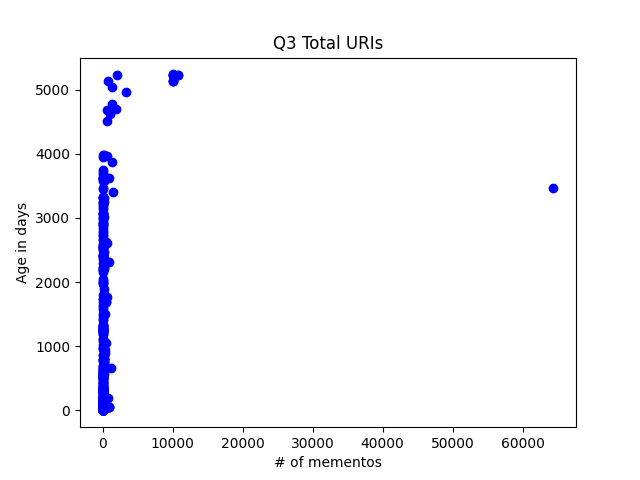
\includegraphics[width=0.95\textwidth]{Final_Scatter.png}
            \caption{Scatterplot with the number of mementos vs. their age}
            \label{fig:my_label}
        \end{figure}

\end{document}
